\chapter{連線教學}
進入防火牆進階設定,並且點選輸入規則後,點選右側的新增規則。\\

\begin{minipage}{\textwidth}
  \centering
  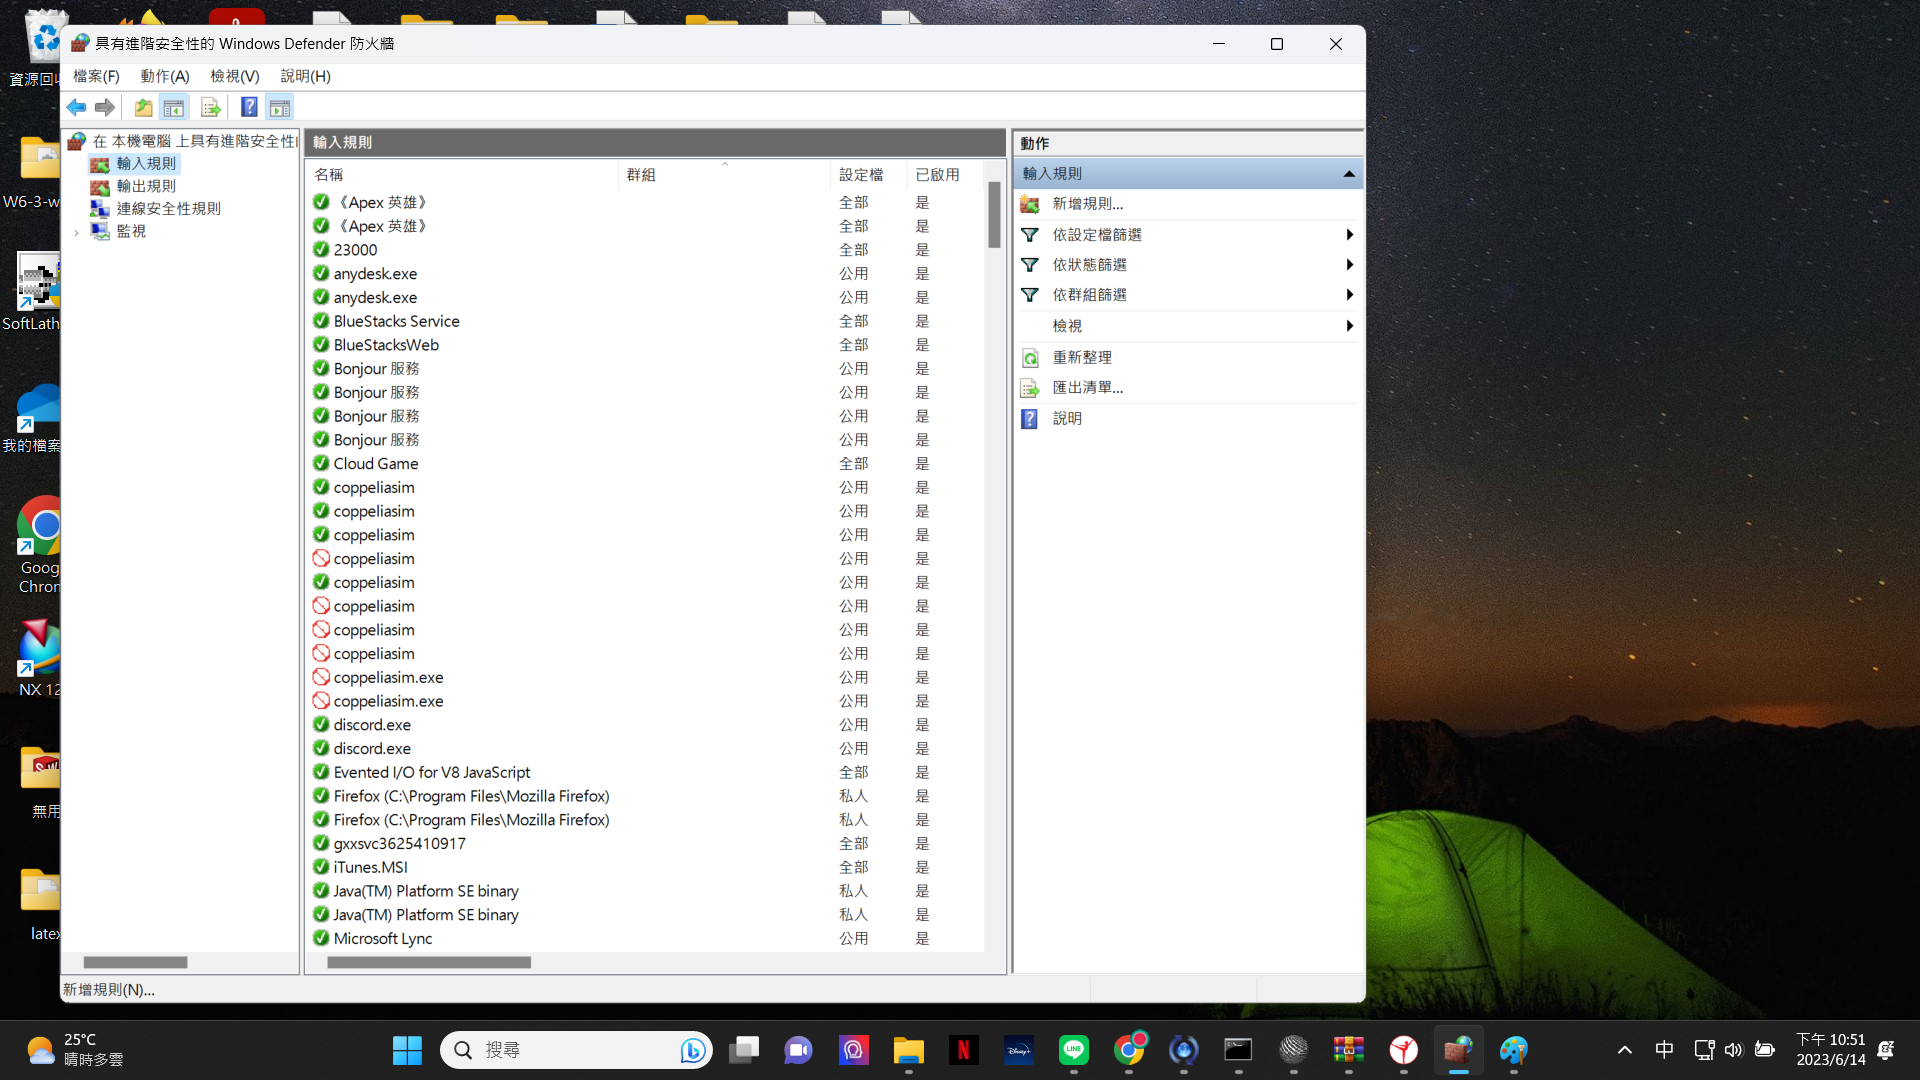
\includegraphics[width=\textwidth]{2}
  \captionof{figure}{連線教學步驟一}
  \label{連線教學步驟一}
\end{minipage}

點選連接埠。\\

\begin{minipage}{\textwidth}
  \centering
  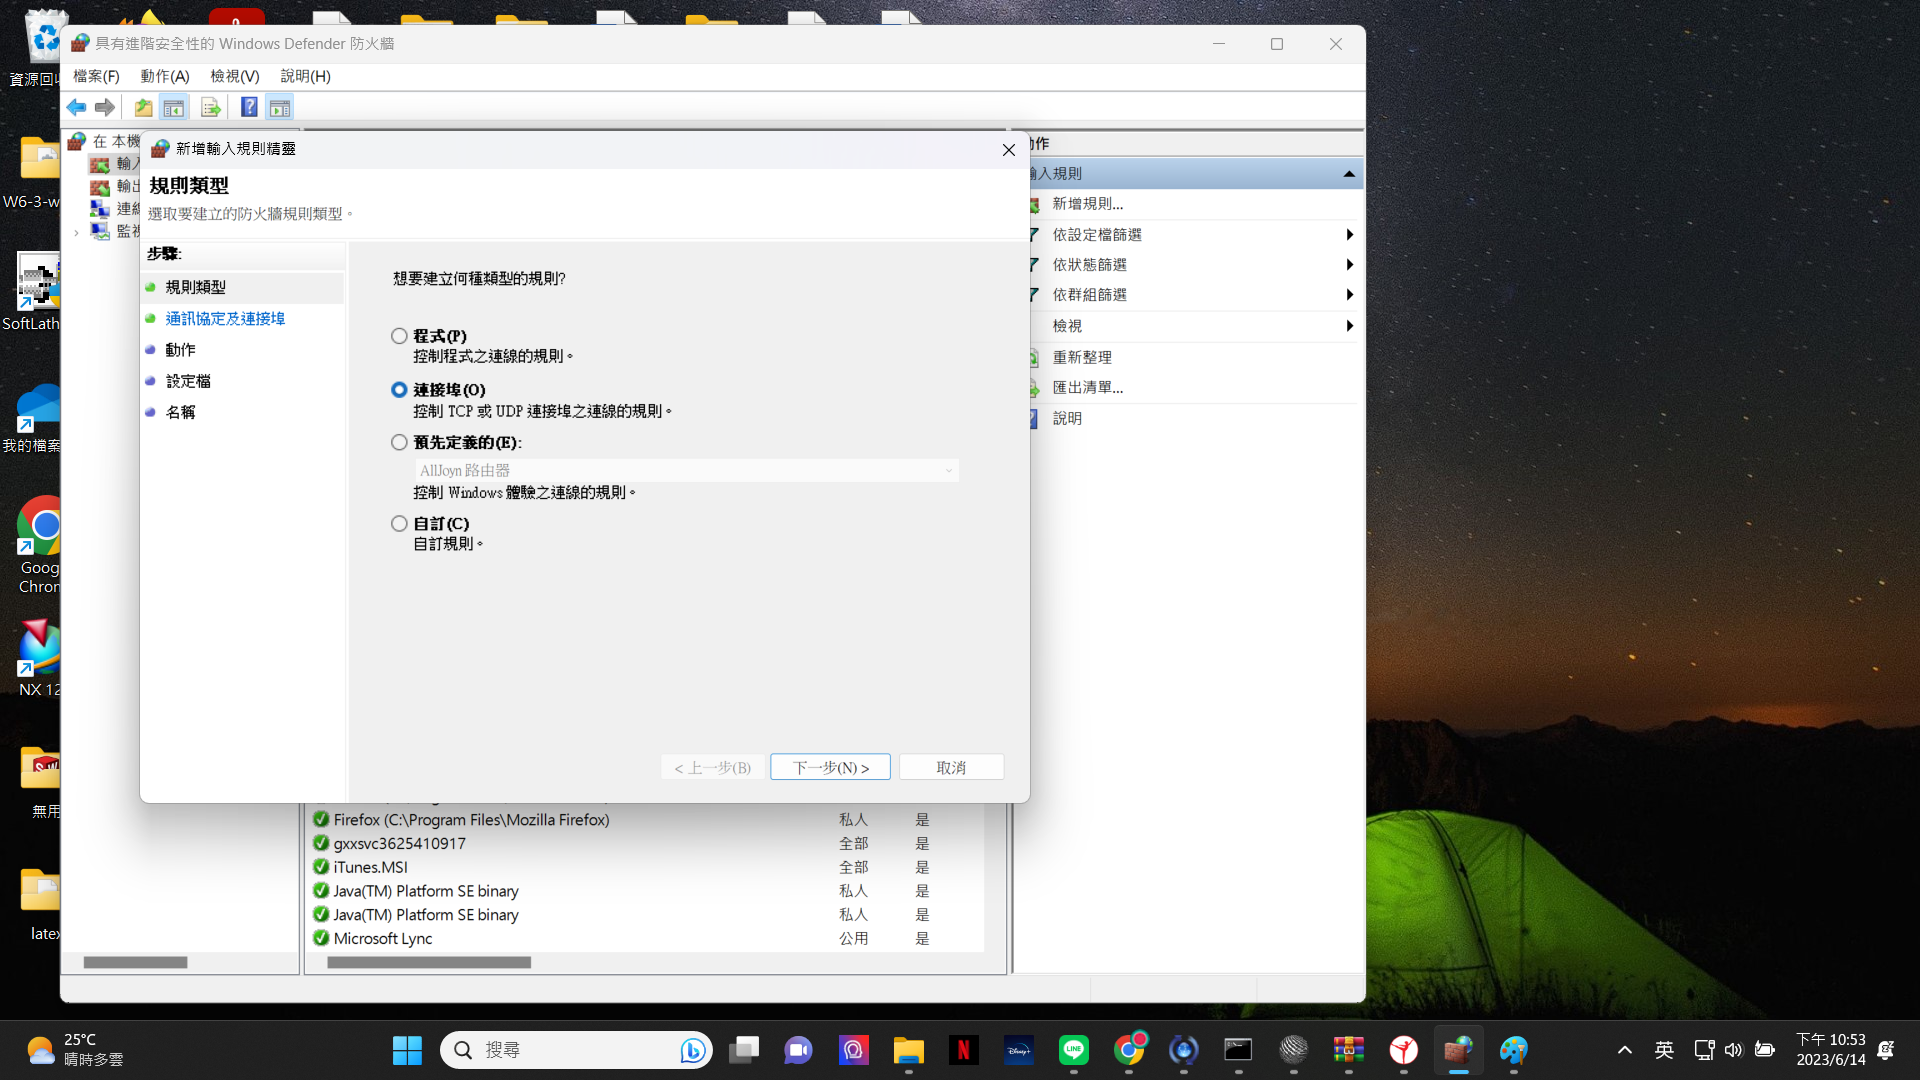
\includegraphics[width=\textwidth]{3}
  \captionof{figure}{連線教學步驟二}
  \label{連線教學步驟二}
\end{minipage}

選擇特定連接埠,打23000-23050。\\

\begin{minipage}{\textwidth}
  \centering
  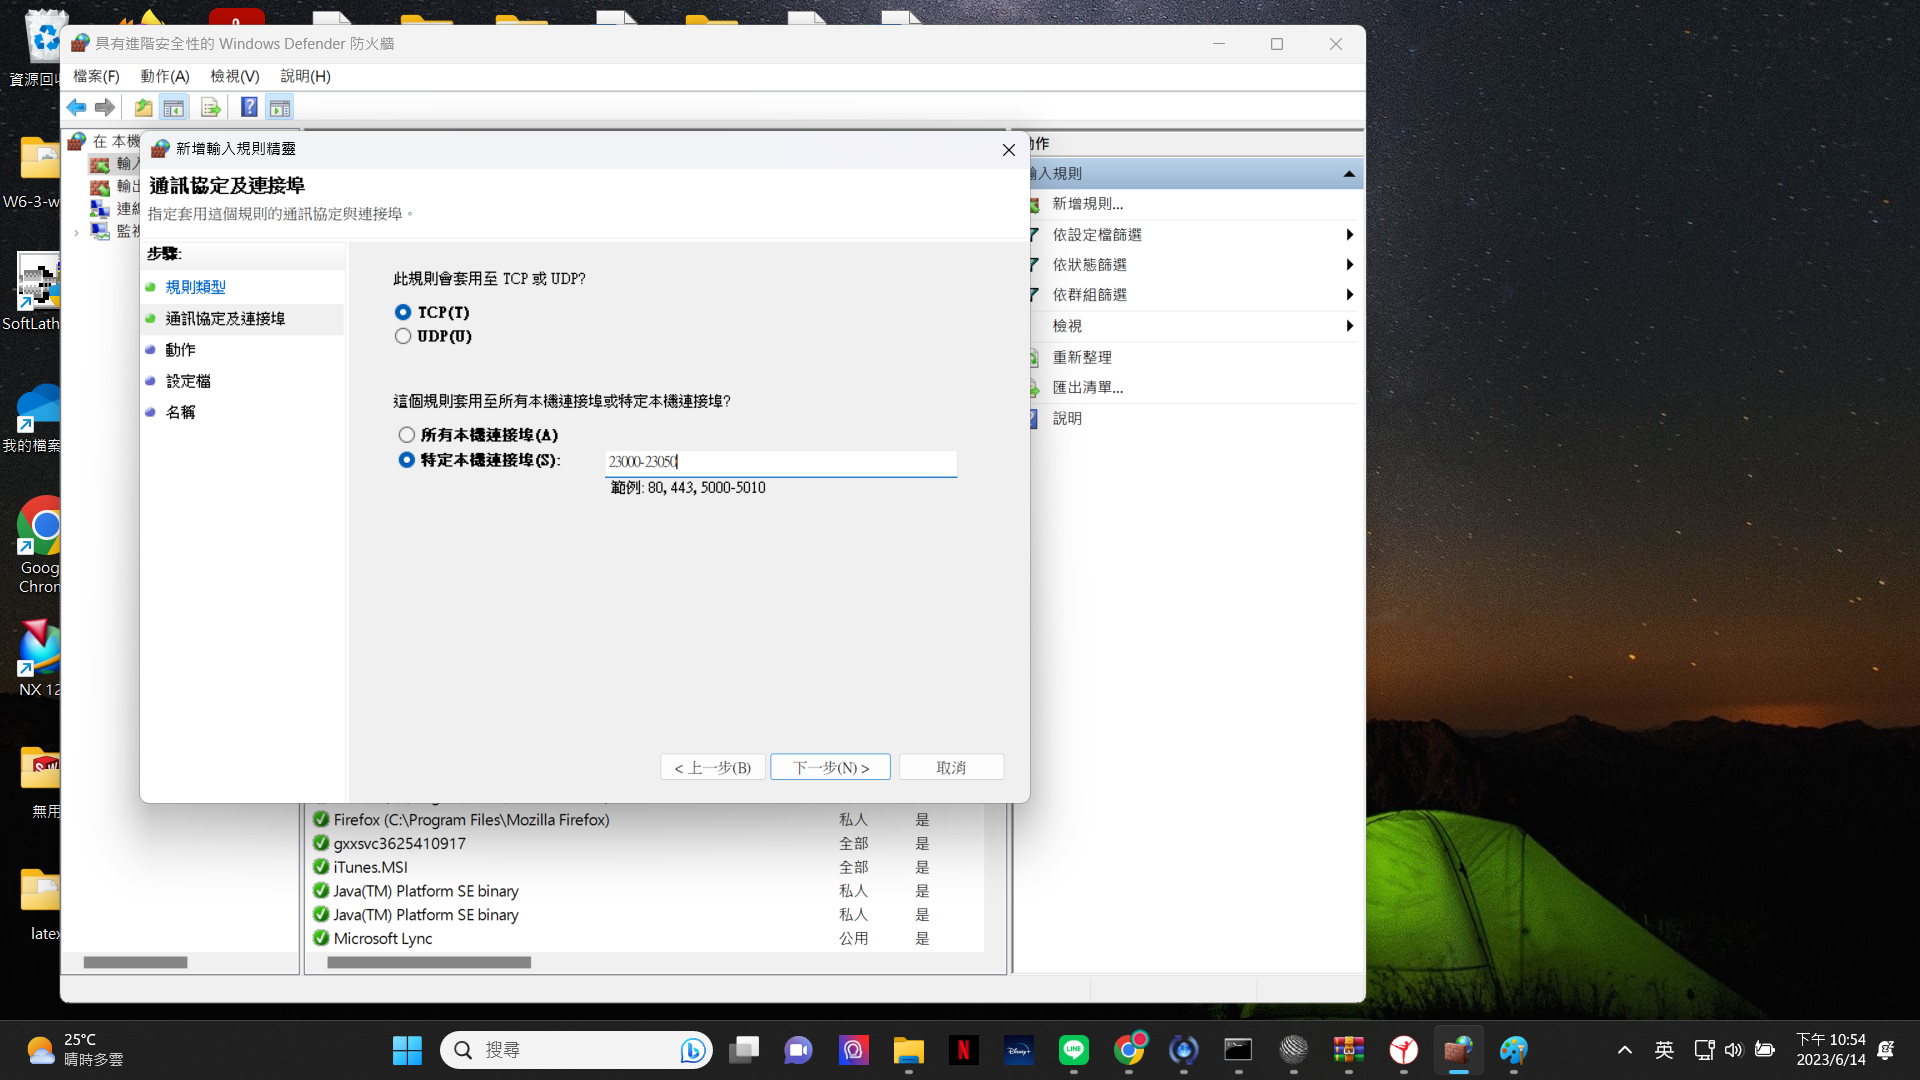
\includegraphics[width=\textwidth]{4}
  \captionof{figure}{連線教學步驟三}
  \label{連線教學步驟三}
\end{minipage}

直接點選下一步。\\

\begin{minipage}{\textwidth}
  \centering
  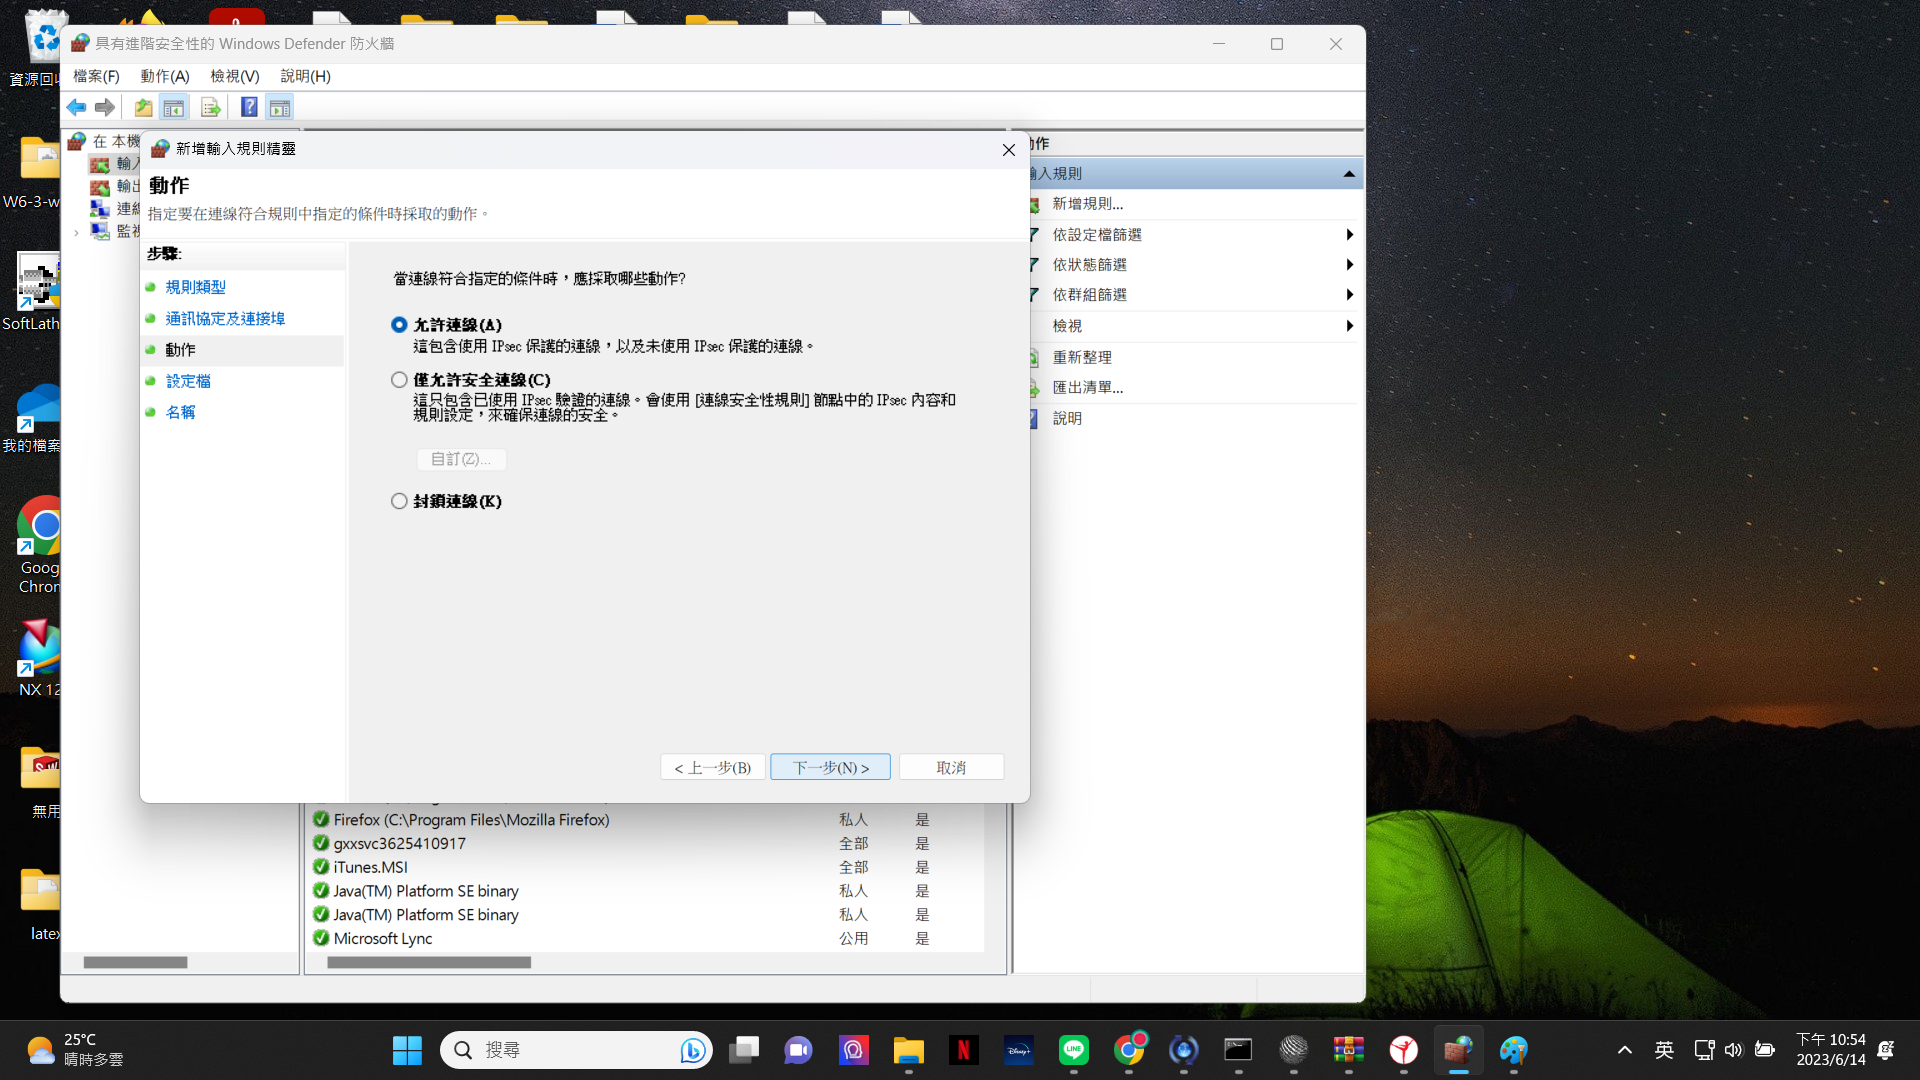
\includegraphics[width=\textwidth]{5}
  \captionof{figure}{連線教學步驟四}
  \label{連線教學步驟四}
\end{minipage}

直接點選下一步。\\

\begin{minipage}{\textwidth}
  \centering
  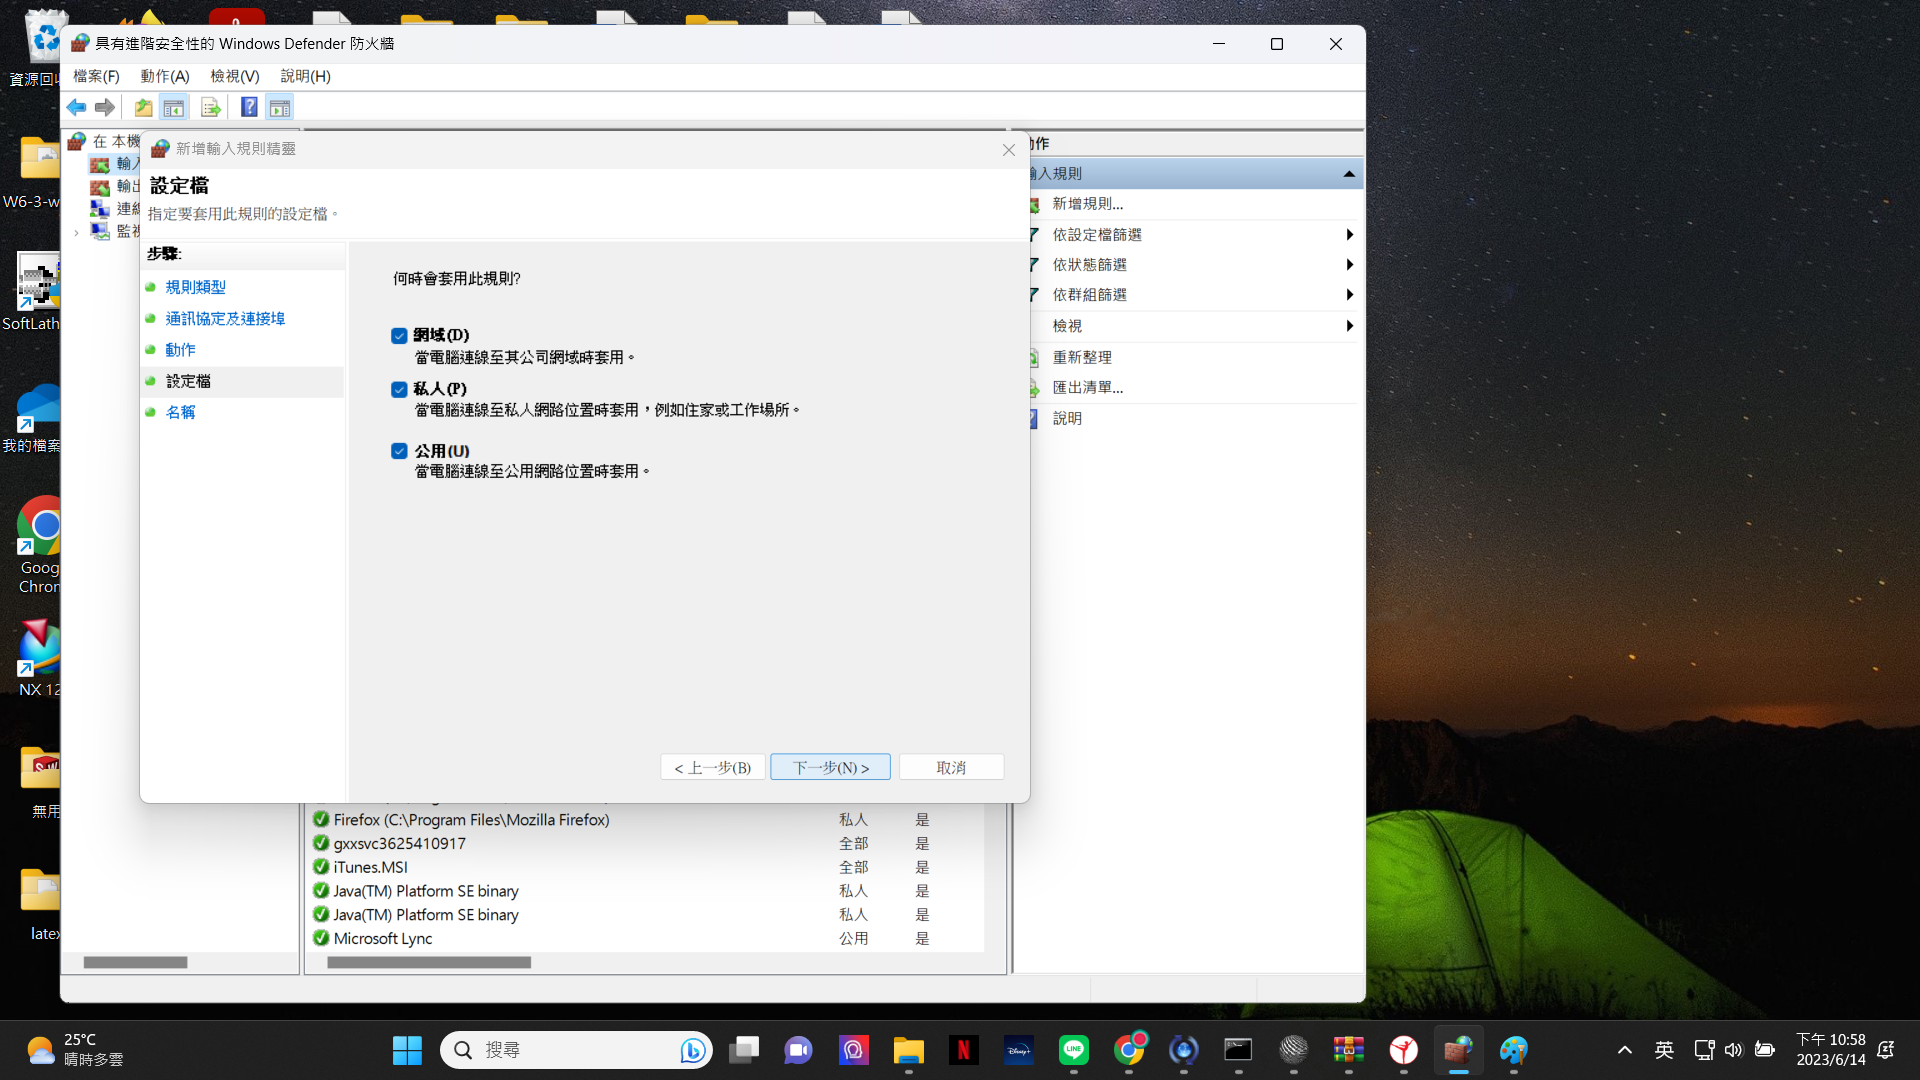
\includegraphics[width=\textwidth]{6}
  \captionof{figure}{連線教學步驟五}
  \label{連線教學步驟五}
\end{minipage}

輸入名稱。\\

\begin{minipage}{\textwidth}
  \centering
  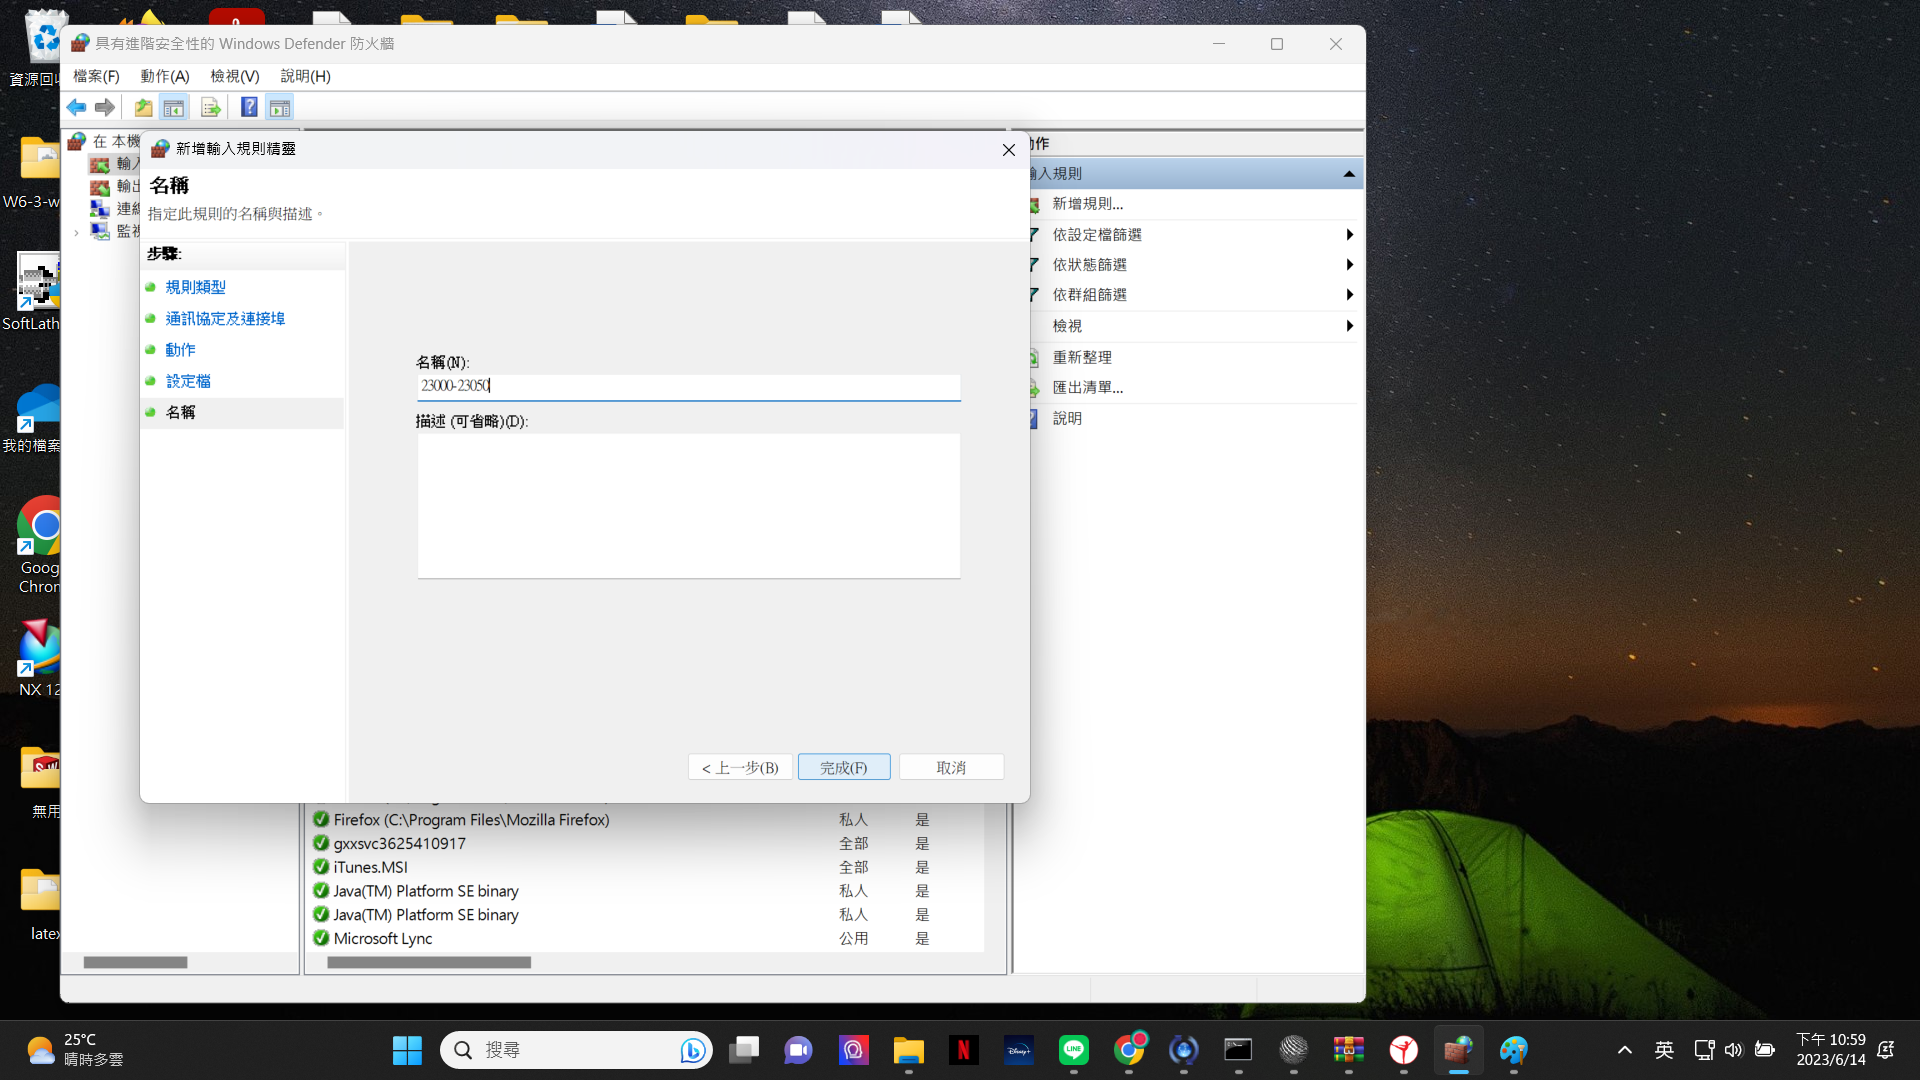
\includegraphics[width=\textwidth]{7}
  \captionof{figure}{連線教學步驟六}
  \label{連線教學步驟六}
\end{minipage}

完成後在列表中就會顯示23000~23050。\\

\begin{minipage}{\textwidth}
  \centering
  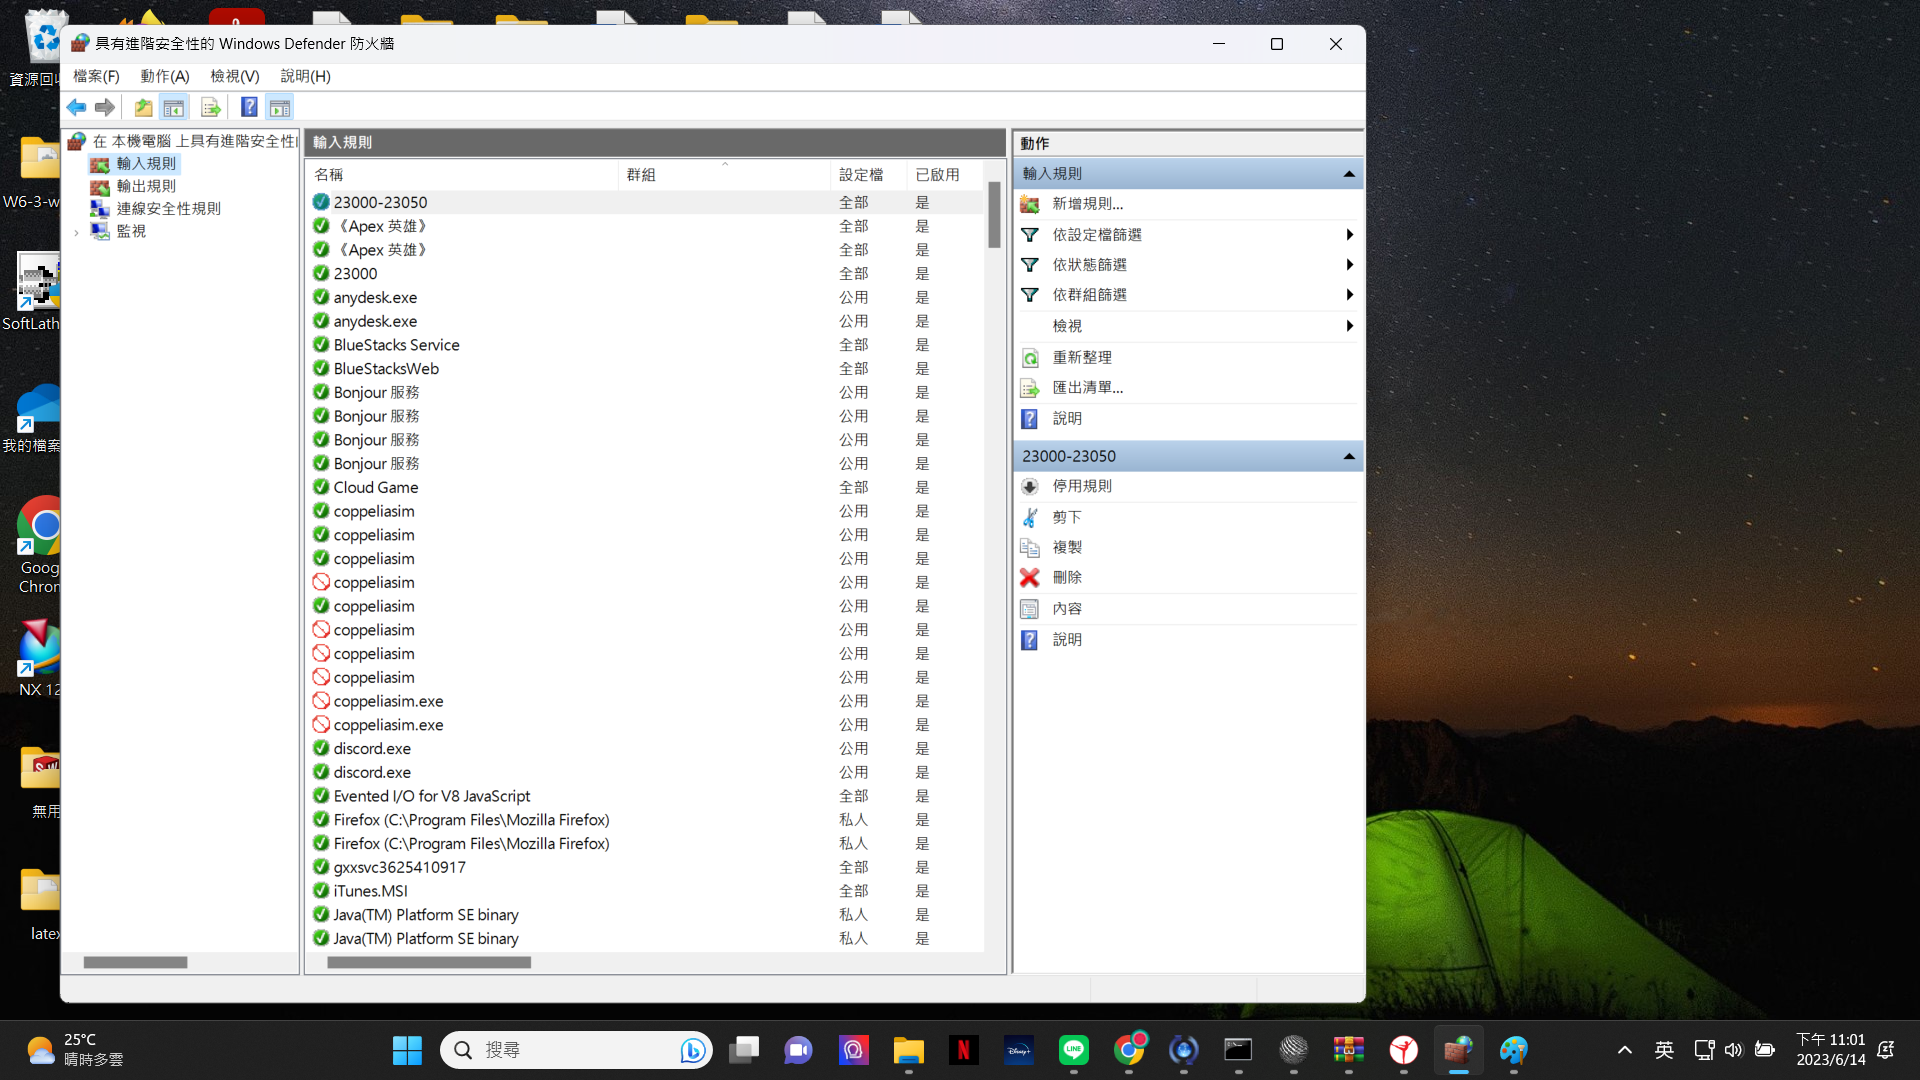
\includegraphics[width=\textwidth]{8}
  \captionof{figure}{連線教學步驟七}
  \label{連線教學步驟七}
\end{minipage}
\newpage
